\chapter{Introduction}
% About Ecommerce 
\paragraph{Introduction to E-commerce}
E-commerce (electronic commerce) is the activity of electronically buying or selling of products on online services or over the Internet. Electronic commerce draws on technologies such as mobile commerce, electronic funds transfer, supply chain management, Internet marketing, online transaction processing, electronic data interchange (EDI), inventory management systems, and automated data collection systems. E-commerce is in turn driven by the technological advances of the semiconductor industry, and is the largest sector of the electronics industry. Modern electronic commerce typically uses the WWW for at least one part of the transaction's life cycle although it may also use other technologies such as e-mail. Typical e-commerce transactions include the purchase of online books (such as Amazon) and music purchases (music download in the form of digital distribution such as iTunes Store), and to a less extent, customized/personalized online liquor store inventory services.There are three areas of e-commerce: online retailing, electronic markets, and online auctions. E-commerce is supported by electronic business. \footcite{wikiecommerce}

E-commerce is fast gaining ground as an accepted and used business paradigm. More and more business houses are implementing web sites providing functionality for performing commercial transactions over the web. It is reasonable to say that the process of shopping on the web is becoming commonplace. E-commerce businesses may also employ some or all of the followings types.
\paragraph{Types of E-commerce} 
The e-commerce industry has made a significant way of selling and buying products.The e-commerce industry can be broken down into two major segments.
	\begin{itemize}
		\item Online stores 
		\item e-commerce platforms
	\end{itemize}
	
\subparagraph{Online Stores} 
An online store is a virtual store on the internet where customers can browse the catalog and select products of interest. The selected items may be collected in a shopping cart. At checkout time, the items in the shopping cart will be presented as an order. At that time, more information will be needed to complete the transaction. Usually the customer will be asked to fill or select a billing address, a shipping address, a shipping option i.e this options are retrieved for the express companies, and payment information. An e-mail or text message is sent to the customer as soon as the order is placed. After the completion of this steps the delivery process is done by the express.

Are websites that sell products online and are one of the most visible segments of e-commerce. One feature of online stores is that they allow smaller companies to build a large audience with less investment than a typical brick-and-mortar store. Because of this, small startups have gained significant traction online even before they had a physical footprint. To better understand online stores we will break them down into different categories based on how they are set up after that we will list the type of online shopping we will be using. The following are the major types of online shopping.
\subparagraph{Business-to-Consumer(B2C)}
The business-to-consumer model of e-commerce represents any business that sells products designed for ordinary consumers on its website. Some of the stores are Amazon\footnote{\url{https://www.amazon.com}}, Walmart sells\footnote{\url{https://www.walmart.com}}. These are all designed for everyday consumers.


\subparagraph{Business-to-Business(B2B)} 
The business-to-business model of e-commerce represents businesses that sell products to other businesses online. Good examples of this are wholesalers, suppliers, and companies selling office products.


\subparagraph{Consumer-to-Consumer(C2C)}
The consumer-to-consumer e-commerce model consists of online stores that serve as intermediaries between consumers. This frequently occurs in the form of auctions or online listings. One prime example of this is eBay, but others include Craigslist\footnote{\url{https://www.craiglist.org}} or Facebook's Marketplace.


\subparagraph{Other}
 A few types of e-commerce stores do not fall under the previously mentioned categories. These tend to be smaller and can include online healthcare exchanges or e-commerce involving the government.

\paragraph{E-commerce Platforms}
The e-commerce platform space covers businesses that offer products and software that support online stores. These companies help store owners run and manage their online business. Companies in this space may sell predesigned shop templates, assist with inventory management, track customer data, and integrate with social media. This space has many facts and is constantly changing with customer preferences.
Shopify\footnote{\url{https://www.shopify}} is a well-known example of an e-commerce platform that caters to small- and medium-sized businesses. Magento\footnote{\url{https://www.magento.com}} and WooCommerce\footnote{\url{https:://woocommerce.com}} also fall under this category. At the enterprise level, Oracle, SAP, and Salesforce are among the growing number of companies that offer e-commerce platforms. Many of these larger companies have made acquisitions in recent years to improve their platforms.

% About Express
\paragraph{Introduction to Express}
The package delivery industry, which consists of small package and express letter shipments,\footnote{For ease of reading, references hereafter to the “package delivery industry” encompass both the small package and express letter services, unless the context clearly indicates otherwise.} has changed dramatically over the years. Radical changes have occurred in the goods transported, the geographic scale of the marketplace, customers needs, the range of service options that carriers offer, and the transportation and communications technology that carriers employ.  The market today bears little resemblance to the market of 30 years ago (at about the time of the Postal Reorganization Act). It bears even less resemblance to the market of 100 years ago (at about the time Parcel Post service began). It is therefore illogical to consider the package market from 30 years ago, or 100 or more years ago, and draw meaningful public policy conclusions for today and for the future. For example, which carrier entered the market “first” is irrelevant for evaluating the potential role of the Postal Service, or any of the carriers, in the modern package delivery market.

Couriers or Express delivery are distinguished from an ordinary mail services by features such as speed, security, tracking, signature, specialization and individualization of express services, and swift delivery times, which are optional for most everyday mail services. As a premium service, couriers are usually more expensive than standard mail services, and their use is normally limited to packages where one or more of these features are considered important enough to warrant the cost. Courier services operate on all scales, from within specific towns or cities, to regional, national and global services. Large courier companies include DHL, Postaplus, DTDC, FedEx, EMS International, TNT, UPS, India Post and Aramex. These offer services worldwide, typically via a hub and spoke model.Couriers services utilizing Courier Software provide electronic Proof of Delivery and electronic Tracking details.\footcite{wikiexpress}

The following provides a brief overview of the various phases of the evolution of the package delivery industry and the key players.  The history of the industry reveals a story of innovation, adaptation, risk-taking and customer demand driving development, with the private sector at the forefront.

\paragraph{The Goal of Guya E-commerce} is to develop a general purpose e-commerce store, the type of the business we follow is Business-to-Customer (B2C) and 	Customer-to-Customer (C2C), where product like clothes can be bought from the comfort of home through the Internet. However, for implementation purpose, this paper will deal with an online shopping for various products (i.e. No media streaming store).

\paragraph{The Goal of Guya Express} sub-project is it's capability of delivering a wide range of parcel for small objects like papers and documents to large objects like furniture and household appliances. On top of that, this system is also able to meet the demand for different parcels like priority and strict storage condition. And by  regarding the city as a whole, this system can perform the delivery more efficiently and save both material resources and manpower resource. At last, Due to the difficulty of testing it in reality, our project is only a preliminary design and view of the picture of future.

\section{Background}
Ethiopia is a developing country and Information Communication and technology are playing their important roles in the development of the country. By E-commerce and Express we mean buying, selling and delivery of any thing products or services over electronic systems such as the internet and other computer networks, with an active delivery system(which of course handled by the express).

The purpose of this document is to define the features of the E-commerce Website/Mobile Application. Here visitors can see the publicly available features such as browse products, view details of products (Size, Color, Cost etc), and view other static contents of site. Registered User can view all publicly available features and in addition to this they can purchase the product by adding them into shopping cart. Website Administrator can mange all the contents and Orders from the Back-end (admin side).

Before attempting to evaluate any e-commerce solution it is necessary to exactly define what is understood as electronic commerce (section What is e-commerce 1.3.1). It is also important to take a look at history in order to comprehend what elements made e-commerce become what it is today (section History of e-commerce 1.3.2). With that knowledge in hand, we will get a glimpse of the future and decide whether the current e-ommerce solutions have a place in it (section Future of e-commerce 1.3.3).

\subsection{What is E-commerce}

As a general definition, commerce is the branch of business that includes all activities, which directly or indirectly are involved in exchanging goods or services. The trade can be held between businesses or individuals, eventually achieving the goal of transferring goods from producers to consumers. When information and communication technologies are applied to support these activities, we are referring to electronic commerce, also commonly known as e-commerce \footcite{Akr11}.

Currently there are four major types of e-commerce (berfily stated in the above section), classified based on the roles involved in the trade: business-to-business (B2B), business-to-consumer (B2C), consumer-to-business (C2B) and consumer-to-consumer (C2C). Other lesser types may involve roles such as government, employee or manager in order to define more specialized e-commerce business models. Though any of those types can be considered to be subtypes of the four major models \footcite{Nem11}.

Besides these four major forms of e-commerce, there are other interesting concepts that have gained popularity these last years: social and mobile commerce. Social commerce is the adoption of social networking features in the context of e-commerce. When it comes to offline shopping, it is a natural practice to gather information from oneself’s personal social networks before purchasing a product. People usually consult their family and friends for advice, and they often speak to the shopkeeper about suitable products. Joining social networks with online stores allows customers to have the same experience, with the advantage of reaching a largest range of people in a shorter time \footcite{GWL11}.

On the other hand m-commerce, an abbreviation for mobile commerce, is any kind of e-commerce activity that relies on the usage of wireless devices, such as cell phones, personal digital assistants (PDA) and smartphones. The range of devices enabled for m-commerce also includes general purpose wireless computers, like tablet and laptop computers \footcite{TNW01}, but are not usually part of research studies. The reason behind that is the existence of hybrid devices between mobile phones and computers, such as smartphones, that are more specifically designed for m-commerce.

\subsection{History of E-commerce}

E-commerce has been gaining more and more relevance in the business context since the moment it was introduced back in the mid-sixties, when the standard that became known as EDI was developed and started replacing traditional mailing and faxing documents. Later in 1979 the British inventor Michael Aldrich invented what he called teleshopping, an early version of online shopping \footcite{Ald10}.

The system consisted of a domestic television connected via telephone line to a real-time transaction processing system, with a shopping transaction program installed. It used a slightly modified television with capabilities to communicate via domestic telephone line thanks to a modem chip originally used in the Prestel system\footnote{System developed by the British public telephone system, whereby news and any text information were received by a television through a telephone line.}. Aldrich’s system was not properly using the Prestel system, but the Prestel data transmission protocol to communicate with computers via telephone line, and therefore to convert televisions into real-time terminals \footcite{Ald11}.

\begin{figure}[!ht]
\center
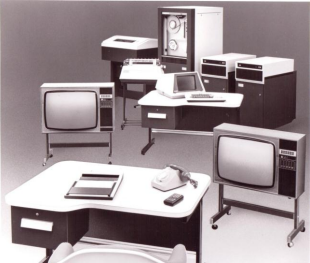
\includegraphics[keepaspectratio]{images/pre-production-online-shopping-1979.png}
\caption{1979 pre-production online shopping system by Redifon.}
%\source{Source: Michael Aldrich Archive}
\label{pre-production-fig}
\end{figure}


Redifon Computers\footnote{Company belonging to Rediffusion Group of Companies.}, the company for which Michael Aldrich was working at that time, started selling this online shopping system (Figure \ref{pre-production-fig}) and installed the first operational application for Thomson Travel Group \footnote{Currently known as Thomson Holidays.} in 1981. Aldrich initially designed his system for B2C online shopping: it worked from an inexpensive domestic television, with simple human interface and using domestic telephone line; despite of that, initial demand was B2B online shopping for holiday travel, vehicle and spare parts, sales, loan finance and credit ratings.

It was in 1984 when Aldrich’s teleshopping system finally reached Jane Snowball’s home, a seventy-two-year-old woman who became the first ever online home shopper when she ordered some groceries from the supermarket chain Tesco (Figure \ref{mrs-snowball-ordering}). The system she used was called GSS (Gateshead Shopping Service), and was part of a social service experiment project in the English city of Gateshead, aimed at elderly people who were not able to go shopping. Another larger project appeared two years later in another city of England, Bradford, for disadvantaged citizens. In both projects it was necessary to develop an early version of what we know today as a cart shopping system \footcite{Ald09}.

\begin{figure}[!h]
\center
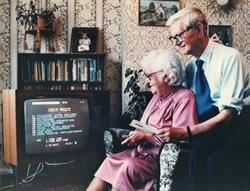
\includegraphics[keepaspectratio]{images/mrs-snowball-ordering-groceries.png}
\caption{Mrs. Snowball ordering groceries from her home in 1984.}
%\source{Source: Michael Aldrich Archive}
\label{mrs-snowball-ordering}
\end{figure}

Elsewhere in Europe similar systems appeared which involved an interactive television using telephone line. Especially important was Minitel system invented in 1982 by France Télécom, that can be considered the most successful of all these early online services. But even in this case teleshopping was only successful in some B2B activities. B2C was not commercially viable due to the difficulty of common people to access the necessary technology. The only working systems were social experiments run by local governments in partnership with supermarkets to deliver groceries to senior and disabled citizens \footcite{BB05}.

E-commerce needed a way to reach a wider variety of people to work, especially outside business-to-business context. Tim Berners-Lee offered that possibility in 1990 when he joined hypertext technology with the Internet creating the World Wide Web [Ber00]. Despite of having the technology, commercial use of Internet was not allowed \footnote{In 1990 most of Internet backbone networks belonged to the National Science Foundation Network. This network was destined to research and educational purposes and had an Acceptable Use Policy that prohibited purely commercial traffic from using it.} when the web appeared. In 1991 this restriction was lifted, but only under the condition of paying a fee according to the usage of the network, which was destined to fund the networking infrastructure. These limitations were also resolved in 1995 when commercial use of the Internet became completely free \footcite{Off93}.

Before that, in 1994 Netscape launched the first commercial browser, with the cryptographic protocol SSL along with it. With the web being accessed by an increasingly amount of people and with a protocol to ensure secure online sales, companies finally had the chance to build a profitable business for B2C in an expanding environment. The first web-shops started to appear, as well as e-commerce solutions built to allow merchants sell online. Only one year later Amazon.com and eBay were born, both considered to be amongst the largest online store corporations nowadays.

Of course all these changes were accompanied by a revolution in payment systems. A series of innovations have been introduced to our daily life during the last thirty years, being the most significant to e-commerce: debit and prepaid cards, online banking and mobile payments via cell phone. All of them contributed to increase the number of payment service providers offered, thus facilitating online payments. Nowadays one of the most important e-commerce payment systems is PayPal, in charge of processing payments between the merchant and the acquirer bank, therefore allowing to send and receive payments securely over the Internet\footcite{KRSS12}.

  
\subsection{Future of E-commerce} us-ecommerce-retail
Despite of being only forty years old, e-commerce has become a very important area in the business environment. Looking back we see the way every technology has changed the e-commerce scenario and given more importance to it. From new protocols to innovative devices, including payment systems and social trends; all has been quickly adopted by companies in order to gain competitive advantage. The introduction rate of new elements in the e-commerce context seems to have grown exponentially over the last few years, as well as the worldwide population involved.

In North America the percentage of digital buyers is currently of 72\% of each Internet user and is expected to grow up to 77.7\% by 2017. A similar growth is expected in Western Europe, with a great difference between northern and southern countries: U.K. and Germany account 87\% and 80\% of e-commerce customers in 2013, respectively, and is expected to grow around 3\%.On the other hand, in Spain the percentage is 54\% and in Italy 44\%, with a predicted growth of 10\%. The highest penetration rate of Internet users in e-commerce will happen in China, where the amount of digital buyers is going to increase 20\% \footcite{eMa613}.


\begin{figure}
\center
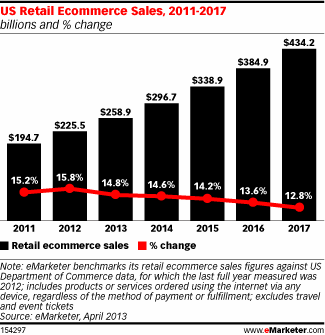
\includegraphics[keepaspectratio]{images/us-ecommerce-retail-from-2011-17.png}
\caption{U.S. retail e-commerce sales from 2011 to 2017.}
%\source{Source: eMarketer, April 2013}
\label{us-ecommerce-retail-from-11-17}
\end{figure}

In number of sales, all major studies foresee a continuous growth in U.S. e-tailing income in the next few years at a compound annual rate that goes from 10\% to 14\%, reaching between \$370 and \$434.2 billion from e-tailing sales in 2017 (Figure \ref{us-ecommerce-retail-from-11-17}) \footcite{eMa413}. When it comes to
Western Europe obtained results are similar with a growth rate of 11\%, reaching even 18\% in southern European countries where the e-commerce market is not yet as mature as in North America [OG13]. Same reason applies to Asia and Latin America with the highest growth rates in the world, around 25\% growth per year. Particularly high are the growthing rates in China and Indonesia, where a 65\% and 71\% is expected in 2013, respectively \footcite{eMa613}.


\begin{figure}
\center
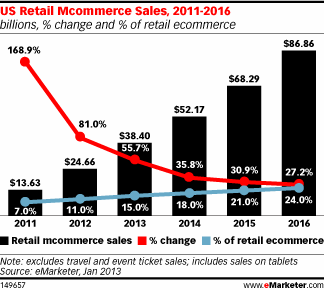
\includegraphics[keepaspectratio]{images/us-ecommerce-retail-from-2011-16.png}
\caption{U.S. retail m-commerce sales from 2011 to 2016.}
%\source{Source: eMarketer, January 2013}
\label{us-ecommerce-retail-from-11-16}
\end{figure}


It is also a fact that mobile devices are being quickly adopted by both merchants and customers, due to all possibilities that they offer in the expanding e-commerce scenario. Some studies show how retail sales made on smartphones will grow from \$8 billion in 2012 to \$31 billion by 2017, becoming a 9\% of e-commerce total sales \footcite{MERJ13}. When tablet computers are also included in the research, m-commerce sales grow from \$24.66 to \$86.86 billions in 2016, having 24\% of retail e-commerce (see Figure \ref{us-ecommerce-retail-from-11-16}) \footcite{eMa113}.

A look at the future of e-commerce reveals a continuous growth in sales and customers, as well as the fast adoption of new technologies such as mobile devices. Therefore it can be expected that new devices and different ways of commerce activities will appear in the near future. It will be therefore necessary for merchants to integrate all their existing e-commerce infrastructure in every context in order to gain advantage from the expected growth.

  
\subsection{Current Alternatives}

Are the current e-commerce solutions ready for bringing quick and affordable integration to future scenarios? Almost all shopping cart solutions offered for online shopping are designer-oriented built web-shops, with multiple plug-in components, customizable options and exchangeable templates. The merchant requires the e-commerce solution to offer a certain feature set in order to use it, otherwise the cost of implementing it may not be worthwhile or simply impossible.

With the raising of cloud computing, many licensed products have move to a more flexible software-as-a-service (SaaS) model, allowing merchants to easily scale their web-shops as their businesses grow. Despite of that, merchants are still very limited to what the software is offering, and depend on the product to evolve in order to expand their e-commerce infrastructure to different environments. Of course, they can also use an independent product to support the missing scenario, but with the high cost of having to maintain two or more different backend data, having to connect them all together.

A very interesting example of these models is Magento, a PHP open-source project that was initially launched in 2008 and nowadays enjoys great popularity. The first version offers a typical out-of-the-box web-shop, highly customizable and with a wide variety of plug-in and templates. The experience of building a web-shop with it was very comfortable, since all the changes were done directly with an administration interface, not requiring any technical knowledge.

Everything was comfortable until the moment the template was not offering a functionality or simply not the way it was needed (e.g. displaying the breadcrumb in a different way or place). In that moment finding the files where the logic that needed to be changed was located became a very hard task and changes were not easy to make either. This experience reflects exactly how developer-unfriendly these kind of models usually are.

Magento also offers a SaaS version of this product, called Magento Go. The experience is even worse, since any kind of customization is limited to what they offer in the administration page, impossibiliting any modification on the code. In 2010 Magento announced the release of the second version, Magento 2.0. This version promised to be more developer friendly, but so far the product has not been released. 


\subsection{What is Express}
\subsection{Early Package Movements}
\subsubsection{Mid-1800\'s to Turn of the Century}
Wells Fargo was founded in 1852. While not the only private express company at the time, Wells Fargo provided a central and colorful role in the early package delivery industry. They created a formidable enterprise for mail and package delivery and banking, especially in the West.\footnote{In the West, "a private express service was safer, surer, and speedier than the federal postal service. 'No one in California mails an inland letter but sends by Express... The miners give their address \& power of attorney to the Express agent who takes their letters out of the post office in San F. twice a month and delivers them to every town \& camp in the placers...'" said Louis McLane, quoted in The American Mail: Enlarger of the Common Life, Chicago: University of Chicago Press, 1972, referenced at page 2 of Stagecoach, Wells Fargo and the American West, Philip L. Fradkin,  Free Press, New York, 2002} In addition to its banking and mail carriage role, it exemplified the early private package industry. One of the founders, Henry Wells, had been a partner in a mail and package delivery business\footnote{Wells defined his earlier company as being in  "the business of carrying parcels and packages as fast as possible, with special care to their safety in transportation and their sure delivery." Id at page 4.} in the East (and even at one time considered acquiring the Post Office\footnote{"Supposedly a monopoly established by law, the Post Office charged high prices for poor service in 1840.  It cost eighteen cents to send a letter from New York City to Troy, New York, but only twelve cents to ship a barrel of flour over the same route. (For longer distances, the letter rate was twenty-five cents.) As a result, private express services who employed messengers proliferated.  They carried the mails at up to one-fifth the cost of the government service.  The Post Office arrested messengers and brought suit against some of the express services.  The harassment didn’t bother the private concerns.  Henry Wells, a partner in an upstate New York express company, proposed that his firm take over the entire postal business of the government and charge five cents for a letter. ‘Zounds, sir,’ reportedly replied an assistant postmaster general to Wells’s proposal, 'it would throw 16,000 postmasters out of office!’  The appointment of postmasters was a major source of political patronage.  Congress did not wish to do away with this 'engine of patronage.' So the solution would have to be an adjustment to the marketplace realities and tightening the monopoly.  The 1845 Postal Act reduced the cost of postage and made the government monopoly on letter mail virtually airtight.  The law, however, was honored more in the breach than observed in the West, where expediency and selective enforcement were the informal laws of the land... Wells Fargo and other express companies became, in effect, opposition post offices."  Id at page 3.}). 

At the time of its founding, the package and banking businesses were unregulated. Mail delivery, however, had been subject to the statutory monopoly of the Postal Service since 1792 and the enactment of the first “Private Express Statutes”.\footnote{"Despite the constant reiteration in the communications of the Postmasters General of the need to prevent private carryings of the mail, it was not until the Postal Act of 1827 that attempts to compete with the federal government in carrying the mail were made criminal." Page 1.27 Towards Postal Excellence, the Report of the President’s Commission on Postal Reorganization, June 1968 Annex III.  But even that did not quell the market forces that responded to the demand for expeditious and reliable service.}

Wells Fargo opened its 12 California offices in 1852 and, according to their promotional material, provided national service: “A typical ad stated that Wells Fargo specialized in shipping ‘gold dust, bullion, specie, packages, parcels, \& freight of all kinds, to and from New-York, and San Francisco” then to other locations throughout the West.\footcite{Stagcoach} Included in their shipments were newspapers, which were carried for free so that other newspapers could reprint the stories, in that pre-wire service time.\footcite{Stagcoach} This helped bind the nation together, and at the same time provided Wells Fargo with free promotion since they often were credited with delivering the news. Historian Carl I. Wheat wrote “Wells, Fargo \& Co’s Express was at this period the most important agency for both express and mail service throughout California and particularly in the mining regions.  By 1858, Wells, Fargo went everywhere, did almost anything for anybody, and was the nearest thing to a universal service company ever invented.  Next to the whiskey counter and gambling table, Wells Fargo’s office was the first thing established in every new camp or diggin’s."\footcite{CLHI}  Wells Fargo was "the single most widespread institution in the early West, being even more omnipresent than the U.S. government."\footcite{PHILPRJ}

Mail and package transport technology was changing rapidly. Coast-to-coast commerce and travel had been provided predominantly by sea. From 1848 to 1858 (from when gold was discovered in California to when the Overland Mail Company inaugurated service\footcite{sfmuseum}) most mail traveled across the continent by steamship with land carriage over the Isthmus of Panama. The travels of Henry Wells from New York to California in December 1852 by boat and then by mule over the Isthmus shows the difficult and perilous nature of that trip.  “By the time Wells reached San Francisco on February 5, 1853, fifteen fellow passengers had been buried along the way and a large number were ill when they disembarked."\footcite{Stagcoach} 1858 marked a significant change to the sea routes with the Congressionally-sanctioned overland stage route that carried mail and parcels. "The first relay of stages, drivers, mules, and horses westward made the grueling, 2,700-mile journey in twenty-four days and nights in September and October of 1858.  It carried the mail and one through passenger.  This was the first true transcontinental mail and passenger service."\footcite{Stagcoach}

Two years later the pony express was founded.  As a service, it was heavy on romance and legend, but short-lived and uneconomic. However, it had to be offered if one wanted the stage business.  “As a profit maker, the pony express was a loser; as a necessity in order to acquire the lucrative transcontinental mail and express business carried by stage coaches, it was a winner; as an indicator of how a new technology could replace an existing one and render the latter obsolete, it was a precursor to what would come later…[the Pony Express] ran for nineteen months and carried light mail from near St. Louis to Placerville, California, at an eventual price of \$1.00 for a half-ounce letter.  At \$23 in current dollars, it was not a service that was affordable for ordinary folks... First undertaken privately and then under government contract, the Pony Express lasted from April 3, 1860, to October 24, 1861.”\footcite{Stagcoach} The overland stage coach mode lasted slightly longer – 11 years.  The mail contract of \$1,000,000 a year did not come close to covering the \$2,425,000 annual expense of the line (1,913 miles, 153 stations, and 2,750 horses and mules).  The shortfall was intended to be made up from express package business and passenger service (which cost between \$225 to \$500 for a one-way throughfare). One of the earliest passengers was Horace Greeley, editor of the New York Tribune and famous for “Go West, young man”, who apparently took the trip in order to promote the development of a transcontinental railroad,\footcite{Stagcoach} which shortly became a reality.

On May 10, 1869, the Central and the Union Pacific Railroads were joined at Promontory Summit, Utah,\footcite{sfmuseum} and it marked the transformation of U.S. goods movement. Wells Fargo continued for some time, adapting to the new mode of mail and package transport.\footnote{Wells Fargo began having its messengers use the railroad. In fact, it advertised that the railroad permitted the country to be crossed in only 4 days, compared to 32 days by stage.} \footcite{Stagcoach}

In fact Wells Fargo’s ability to successfully adapt to the use of railroads became a threat to the Post Office that later caused Wells Fargo to withdraw from the express mail business.  "...Wells Fargo continued to perform that function so essential to the smooth functioning of a democracy: delivering the bulk of the mail west of Salt Lake City and Albuquerque.  The inevitable confrontation between Wells Fargo and the U.S. Post Office Department in 1880 was a classic example of a private business competing directly and successfully with a government agency... During the Gold Rush era and shortly afterward, Wells Fargo’s private mail system was tolerated because the government recognized that it did not have the same broad reach or the same degree of efficiency."\footcite{Stagcoach}  A temporary compromise was reached whereby mail carried by Wells Fargo directly would pay double postage: the stamp price, plus the Wells Fargo charge, and customers were willing to accept the higher cost because of the quality of the service. “In this way, the government got its due and the customer got quicker service."\footcite{Stagcoach} This arrangement held for a while, but the company ultimately had to abandon the mail business towards the end of the 19th Century.\footnote{"On May 24, 1895, Wells Fargo quietly removed all its collection boxes in San Francisco and on the next day announced it was ending its letter service."}  "In the old days... [Wells Fargo] not only competed successfully with the Government, but we beat the postal system at every turn of the road, but now the Federal authorities have adopted all of our plans, and they do the work as well as we do."\footcite{Stagcoach} \footnote{Note that the withdrawal was from letter mail; the company remained in the express package business and in banking.}

\subsubsection{Early 20th Century: Railway Express Agency (REA), UPS, and Parcel Post}
UPS Ground Service  In 1907 two Seattle teenagers (Jim Casey \& Claude Ryan) started the American Messenger Company, whose messengers ran errands, delivered packages, and carried notes, baggage, and trays of food from restaurants. They made most deliveries on foot and used bicycles for longer trips. Only a few automobiles were in existence at that time and department stores of the day still used horses and wagons for merchandise delivery. The company was soon delivering small parcels for local department stores and changed its name to Merchants Parcel Delivery. The company expanded outside Seattle in 1919 with the acquisition of Oakland based Motor Parcel Delivery and was renamed United Parcel Service in 1930. In the early 50\'s UPS began the process of expanding its services by acquiring "common carrier" rights for the entire country. 

Parcel Post  Parcel Post service became available on January 1, 1913, and constituted an expansion of a more limited package service of the Post Office.\footnote{www.postalmuseum.si.edu For example, in 1907, merchandise under four pounds could be sent by the Post Office for sixteen cents per pound.  Even then, however, the discrepancies in sub-categories of service were irreconcilable: domestic shipments from any city in the U.S. to New York City would cost sixty-four cents, but if it were destined to one of the thirty-three countries then served, and by chance went through New York City, the rate was twenty-five percent cheaper -- forty eight cents. (Address by Postmaster-General Meyer to the New England Postmasters\' Association, Boston, October 1907, as referenced by Charles W. Burrows, Further Thoughts on Parcels Post,  Selected Articles on the Parcels Post, Second and Revised Edition, compiled by Edith M. Phelps and published by The H.W. Wilson Company, Minneapolis, 1913)}  Prior to 1913, farmers had to convey their produce to the nearest town large enough to support a [private] express office, which added to the price of transporting their goods to the city. But with the combination of Rural Free Delivery (RFD) and Parcel Post, package service was provided from their mailbox.  As discussed below, there is debate regarding Congress’ intention about how broad this competitive offering would be.

Parcel Post service expanded rapidly and, due to its pricing and availability, was widely used, and even sometimes abused.  The Smithsonian Institution’s Postal Museum notes two particular amusing instances: one in which an entire bank was shipped, brick by brick, and another case where a child was transported by Parcel Post because her parents found the rates cheaper than passenger service.\footnote{"By far the largest object ever moved through the Parcel Post System was a bank. Not all at once, of course, but practically brick by brick. When W. H. Coltharp, in charge of building the Bank of Vernal, Utah... The bricks which Coltharp wanted were produced by the Salt Lake Pressed Brick Company, located 427 miles from Vernal. Instead of paying four times the cost of the bricks for them to be shipped by wagon freight, Coltharp arranged for the bricks to be shipped in 50-pound packages, through the Parcel Post Service, a ton at a time. The Salt Lake City and Vernal postmasters as well as the Uintah Railroad, all responsible for hauling the bricks became frantic as tons of bricks piled up... .In the end, all 40 tons of bricks were delivered for Coltharp's bank."}

The legislation establishing the Parcel Post service appears to have been intended as a narrow response to a perceived gap in service: The Congressional Record reveals that the purposes of Congress in establishing parcel post were:
\begin{itemize}
	% numeric
	\item To provide a transportation service for small parcels (not over 11 pounds or 72 inches in length and girth) extending beyond that supplied by express companies and other carriers.
	\item To give the farmer an opportunity to sell his products direct to consumers.
	\item To enable residents of rural districts and small communities to receive small quantities of merchandise by mail from merchants in what were then distant cities.
\end{itemize}

In establishing parcel post for those purposes, Congress also made clear its intentions that:
\begin{itemize}
	% numberic
	\item Rates should produce revenue adequate to cover costs.
	\item Government should not unnecessarily compete with private transportation.
	\item Parcel post should supplement not supersede private carriers.\footcite{REA1}
\end{itemize}

That view was reinforced later by several Congressional Committees.  On October 19, 1951, Senate Report No. 1039, 82nd Congress stated that "the benefits of low-cost service are illusory if part of the total cost of transportation is borne by general taxpayers. If shippers do not pay the full cost of the transportation service they use, traffic generally is diverted from transportation media inherently better able to serve them.” On a similar note, the House Committee on Post Office and Civil Service issued a report that “[i]t is apparent that the problem of the Government agency competing with private business to the point that that private business, the Railway Express Agency, is being irreparably damaged cannot be met by rate increases alone however, it can be met by a return in part to the size and weight limits originally approved by Congress when parcel post was established to provide a small parcel delivery service to areas which are not serviced by other transportation facilities. "\footcite{Stagcoach}

\paragraph{Railway Express Agency (REA)} As World War I ended, "the reality of a declining business competing with the Post Office [for parcel shipments] and overseen by government regulators forced Wells Fargo and six other express companies to the bargaining table"\footcite{Stagcoach} for the creation of the Railway Express Agency (REA). 

For over 56 years, the REA moved the nation's packages and freight. Its green trucks and rail cars were a welcome sight to anyone expecting a package. It was the railroad equivalent of today's modern package delivery companies, such as UPS and FedEx.   In 1929, the nation's railroads bought the express business. In return for a monopoly on the movement of traffic on passenger trains, the express company was obligated to accept any and all shipments destined anywhere in the U.S.  In its peak of success, REA employed over 45,000 people in 23,000 offices and operated over 190,000 miles of railway lines.  In addition, over 14,000 miles of shipping lines, 91,000 miles of air routings and 15,000 miles of trucking lines were traveled by REA shipments.  Seventeen thousand trucks handled over 300,000 separate shipments daily, ranging from small packages to carload-sized lots.
Despite REA's early successes, the railroads became less relevant to express delivery and REA did not change its business model to adapt. On February 21,1975, the Company filed for bankruptcy protection.  REA stated several reasons for the bankruptcy petition, including losses created by years of railroad domination, a high rate of inflation, a recent decline in express shipments, and limited availability of credit.

\subsubsection{Development of Modern Surface and Air Networks (Late 20th Century)}
The establishment of the Interstate Highway System in 1956 to build a transcontinental network of superhighways, the enactment of airline deregulation in 1978, interstate trucking deregulation in 1980, and intrastate trucking deregulation in 1994 contributed to the significant shift to truck and air transport, especially during the latter part of this period, and marked the growth of the modern package delivery industry.  The charts in attachment A show the rapid development of the industry, with more than a 36-fold increase between 1960 and 19981.\footcite{PRC} The development of modern surface and air networks in the U.S. is demonstrated by UPS and FedEx.

\paragraph{UPS Air Operations} In 1929, UPS opened United Air Express, offering express package delivery via airplane to major West Coast cities, and as far inland as El Paso, Texas. Due to the 1929 stock market crash and a failing economy, the air service was discontinued after only eight months. In 1953, UPS resumed air service, offering two-day service to major cities on the East and West coasts. Packages flew in the cargo holds of regularly scheduled airlines. Called UPS Blue Label Air, the service grew until by 1978 the service was available in every state, including Alaska and Hawaii.  In 1988 UPS received authorization from the FAA (Federal Aviation Administration) to operate its own aircraft, thus officially becoming an airline.\footcite{uspsManual}

\paragraph{Federal Express (FedEx)} While the USPS was the first to deliver urgent letters, it has many current rivals because its monopoly power is not monolithic. The Postal Service is authorized to adopt suspensions to the Private Express Statutes for specific circumstances in which the public interest might be best served by a private carrier.1 It is under such authority that Federal Express, UPS, and other carriers conduct their express letter operations.

Federal Express was incorporated in June 1971, and officially began operations on April 17, 1973, with the launch of 14 small aircraft from Memphis International Airport. On that night, Federal Express delivered 186 packages to 25 U.S. cities - from Rochester, N.Y. to Miami, Fla. The company was named Federal Express because its founder, Fred Smith, was working on obtaining a contract with the Federal Reserve Bank and, although the proposal was denied, he believed the name was appropriate for express envelope and small package delivery.  Profitable in the U.S. market by July 1975,\footcite{uspsManual}  \footcite{nalcManual} Federal Express grew rapidly in the international market when it acquired Tiger International, Inc. (also known as Flying Tigers) in February 1989.  Two further acquisitions were of substantial significance:  In 1995, Federal Express acquired Evergreen International Airlines, Inc.'s all-cargo route authority to serve China.  The other was when the company acquired Caliber System, Inc., in January 1998 which gave FedEx ownership of RPS, a major ground package carrier (now designated as FedEx Ground).\footcite{fedexHistory}

It was during this period that the industry saw the introduction of many new services and service enhancements.  Package carriers began to offer multiple delivery options, including same day service, next day delivery, and a variety of deferred, time-specific delivery options.  Delivery guarantees accompanied express movements.  Private carriers then expanded these guarantees to more traditional "ground" movements in the late 1990\'s.

As the scale of commerce progressed from local communities to national trade, then to global markets, the industry followed suit, with the heavy capital investments needed to expand.  This period also produced intense competition as private carriers achieved 100\% geographic coverage of the United States and to most points of commerce around the globe.

Significant investments in information technology enabled package carriers to provide to customers the ability to track a package’s movement from origin to destination.  Other advances included combining logistics, freight and financial services with traditional package delivery in order to offer customers full supply chain management solutions.  

The development of the package industry has enabled others to innovate.  Michael Dell (Dell Computers) and Jeff Bezos (Amazon.com) are but two of many innovators that have used just-in-time deliveries, coupled with the power of the e-commerce, to launch new business models. Those innovations helped contribute to the relative importance of the package delivery industry that carries, by some estimates, goods valued between 8.6\% and 14.3\% of the nations Gross Domestic Product.\footcite{JRCEC}

\section{Problem Statement}
Most of our country people purchases and pickup items, documents, news paper and foods by going to store front, even-though there are some e-commerce site that partially provide online purchases. By doing some digging we found some major concerns about the site/mobile apps that provide this kind of services below we’ll try to illustrate what we believed to be the factors affecting it.

One is that E-marketers not knowing the factors affecting online Ethiopian behavior, and the relationship between these factors and the type of online buyers, then they can further develop their marketing strategies to convert potential customers into active ones. we brief how we conduct the research and the methodology we will use more in the Tools and methodology section.

\begin{itemize}

	\item Products listed in some of the already made e-commerce sites are not what they say or look like. 

	\item Companies in Ethiopia that provide delivery service their calculation of cost of delivery is not fixed it is more of ranged by kilometers e.g 1-3 km 50 Birr 3-7 km 75 Birr and above 7 km 100 Birr this kind of cost analysis is not fair for customer with minim kilometers.

	\item Lack of website's Lowest Denomination Design :-The websites made doesn’t consider old phones but instead trays to keep up with new phone, from the perspective of the rapid change(developing) of technology is a wonderful thing, but due to t majority of Ethiopian peoples use old phone/browser even those technologies are outdated.

	\item Live GPS Parcel Tracking :- No body knows where their parcel is and how much time it take to reach the destined place (No Live Tracking).

	\item No Return Policy/Service :- Once you bought you bought it, their is no returning it weather the parcel is damaged, it is not the item you expected, opened or have some cracking while delivering.

	\item No Customer Live Chat Support

	\item Drawback of the Inventory System

	\item Limited payment service :- Cash On Delivery (C.O.D)

\end{itemize}

\section{Objective}

\subsection{General Objective}
In this sub-project (i.e Guya E-commerce) is to reduce the labor-full way of shopping and
delivery service to more enjoyable way, more rich experience of user interface, cut
the time and cost of shopping and delivering method.

In this sub-project (Guya-Express), our aim is to design a uniform parcel delivery system in Ethiopia which can offer service to all kinds of customers in the city including manufactures, department stores, restaurants, individual people, and most importantly for Guya-E-commerce and so forth.

\subsection{Specific Objective}
\begin{description}
	\item[Enhance customer service :-] As the system is automated and online based customers will have less of problems and enjoy a hassle free shopping experience.
	\item[Advertising savings :-] As the web platform provides greater reach it minimizes advertising and marketing cost.
	\item[Increase the level of customer service :-] by avoiding under stocking of products so that the store never runs out of stock. Easy to determine products which are understock and restocking them.
	\item[Impose Data Security :-] so that unauthorized individual cannot access sensitive data and
cause mishaps which might disrupt the system.
	\item[Data loss is minimized :-] as data is saved in database and periodic backup is done. So in case of any disaster data can instantly be restored.
	\item[Maximize customer reach :– ]As the website is a global platform the potential customer base increases as more user access the website from anywhere around the world.
	\item[Localization :-] Multiple language support, local Time and Date support (conversion).
	\item[GPS Tracking :-] Live GPS tracking for Parcels.
	\item[Shop Comparison :-] It's easy to do comparison shopping online and learn from product reviews written by other shoppers.
	\item[Variety of payment methods :-] Payment can be initiated by Cash On Delivery (C.O.D), Mobile Wallet, or Bank Transaction.
	\item[After-sales Service :-] E-shopping also provide after-sales service in which customer problem is solved.
	\item[Data security :-] Data security is maintained to a relatively high level by implementing it at the Database level, so as to ensure that only authorized users have access to confidential client information.
	\item[Enhance customer service :-] As the system is automated and online based customers will have less of problems and enjoy a hassle free shopping experience.
	\item[Advertising savings :-] As the web platform provides greater reach it minimizes advertising and marketing cost.
	\item[Suspicious activity detection :-] If a certain user/computer try to guess password and username more than the limited state, the computer's IP address will be captured for further analysis.
	\item[Banning items :-] Banning items that may contain copyrighted item, sexual items, abnormal posts through either manual or Natural Language Processing.
	\item[Text Message Integration]
	\item[Cookie based suggestion]
	\item[Inventory Forecasting :-] Automatic Warehouse product stocking identification
	\item[AI based recommendation engines]
\end{description}

\section{Scope}
The scope of the project will be based on the features and functionalities of the website. The Project website and mobile application functionalities are listed below :-
\begin{itemize}
	\item Advanced Search :- Search suggestion with multiple language, from specific category search. 
	\item Search Engine Optimized :- is the process of increasing the quality and quantity of website traffic by increasing the visibility of website or web page to users of a web search engine.
	\item Product Filter :- Filtering products by price, brand, model, rate, review, most viewed, popular, deal of the day
	\item Control Panel for different actors
	\begin{itemize}
	    \item Website Administrator
	    \item Customer
	    \item Customer service etc...
    	\end{itemize}
	\item Inventory System :- is for tracking inventory levels, orders sales and deliveries.
	\item Shopping Cart	 :- Buying multiple items once
	\item Check out :- For selecting billing method, shipping address
	\item Email Service :- Account Verification, Password Reset, Notification, Receipt, News Subscription, Marketing Promotion)
	\item Phone Number Integrated Service :- Account Verification, Password Reset, Notification, Semi Receipt, Semi News Subscription, Order Placement  Notification
	\item Delivery(Parcel) Tracking :- Seeing the location the parcel is now
	\item Frequently Asked Question (FAQ)
	\item How to use the site :- Suggest on how to use the site on first visit of the site
	\item Delivery between two parties :- document, gift, money from one to person to another.
	\item 3rd party Delivery for any E-commerce platforms (i.e. cross site API calls)
	\item Feedback services for customers :- Customer feedback is the process or specific instance of providing information to businesses about products, services and customer service.
	\item Different Payment methods
\end{itemize}

\section{Limitation}
\begin{itemize}
	\item Lack of touch and feel of merchandise in online shopping. Lack of touch-feel-try creates concerns over the quality of the product on offer. Online shopping is not quite suitable for clothes as the customers cannot try them on.
	\item Lack of close examination in online shopping.
	\item Limitation of to use online payment. Ethiopia banks use debit card and automated teller machines (ATM) but have not begun to issue credit cards.
	\item Most Ethiopians do not have credit card, Mobile Wallet.
	\item Slow internet connections 
	\item Expensive and unreliable internet connection.
	\item Limited Bank-to-Bank integration.
	\item Tax Calculation :- Since there is no rules on E-commerce that governs tax calculation we will make tax calculation by the same taxation rate as retail store.
	\item Cost of buying equipment, principally the hardware like barcode reader, GPS tracker 
\end{itemize}

\section{Assumptions and Dependencies}
These factors are not design constraints on the software, but rather assumptions on which the requirements have been based. Any changes to these assumptions affect the requirements stated herein. If these assumptions are not true, these requirements cannot be considered valid. For this reason, the requirements are said to be dependent on these assumptions

The following assumptions have been made about the system.

The project focus on providing Shop and Deliver through the internet. So our assumption is the followings
\begin{itemize}
	\item Internet facility
	\item Any retailer have a printer or have access to one for printing labels
	\item Any retailer have measuring equipment or have access to one for weighting and measuring parcels
\end{itemize}

\section{Significance Of The Project}
Since the proposed system is hosted in the internet it will allow customer from all over the world to access the system. The customers will face hassle free shopping as they do not need to be physically in the shop to buy a certain item. Since the payment is done online or cash on delivery it is more convenient for the consumers. The management and maintenance of the information in the system will be more efficient and effective as a result will be much more time effective. The proposed system will help system users to get
desired information within a short period of time. Administrative authorities can efficiently get desired report about Clients, products, orders, payment and delivery.

\section{Tools and Methodology}
\subsection{Data Collection Methodology} 
Our front-end design principle is lowest denomination design so we will be conducting data collection for our project through some of the methods listed below with pros and cons for the project.

\paragraph{In-person Interview}

\begin{itemize}
    \item[$-$] Pros :In-depth and a high degree of confidence on the data
    \item[$-$] Cons : Expensive, time
\end{itemize}

\paragraph{Mail Surveys}
We will be using main surveys for reducing cost of paper and printing, and for those that we can not reach physical.
\begin{itemize}
    \item[$-$] Pros : Can reach anyone and everyone – no barrier
    \item[$-$] Cons : Expensive, data collection errors, lag time
\end{itemize}

\paragraph{Phone Surveys}
Same as the Mail surveys we will be using main surveys for reducing cost of paper and printing, and for those that we can not reach physical.
\begin{itemize}
    \item[$-$] Pros :High degree of confidence on the data collected, reach almost anyone
    \item[$-$] Cons : Expensive
\end{itemize}

\paragraph{Web/Online Surveys}
As to our knowledge the is not sufficient data.
\begin{itemize}
    \item[$-$] Pros : Cheap, can self-administer, very low probability of data errors
    \item[$-$] Cons :Not all your customers might have an email address/be on the internet, customers may be wary of divulging information online
\end{itemize}

\paragraph{Questionnaire Surveys}
Is a research instrument that consists a set of questions or other types of prompts that aims to collect information form a respondent.
\begin{itemize}
    \item[$-$] Pros : Relatively fast, Responses are gathered in a standardized way,\\information can be collected form a large portion of a group
    \item[$-$] Cons :Low response, Respondents may not be able to read the question or potentially not understand, answers may be incomplete or irrelevant
\end{itemize}

\paragraph{Observation}
Observation, as the name implies, is a way of collecting data through observing. Observation data collection method is classified as a participatory study, because the researcher has to immerse herself in the setting where her respondents are, while taking notes and/or recording.
\begin{itemize}
    \item[$-$] Pros : Very Cheap, flexibility, direct access to data
    \item[$-$] Cons : Time consuming, impact of observer on primary data\footnote{In a way that presence of observer may influence the behavior of sample group elements.}
\end{itemize}

Questionnaire, Phone Surveys, Mail Surveys, In-person Interview are administered in order to inquire form general populace. In total 100 to 200 will be administered using some of the methods listed above based on the cost analysis made.

\subsection{Programming Language And Database Tools}
\paragraph{Front End:}
For designing the structure of the project following technologies are used:
\begin{description}
\item[HTML5 : ] Is a markup language. HTML5 is used to create electronic documents (called pages) that are displayed on the World Wide web (WWW). Each page contains a series of connections to other pages called hyperlinks.
\item[NODEJS : ] Node.js is cross-platform, javaScript runtime environment that executes JavaScript code outside of browser. It lets used of JavaScript to write command line tools and for Server-side scripting\footnote{running scripts server-side to produce dynamic web page content before the page is sent to the user's web browser}
\item [JAVA : ] Mainly for android application development.
\item [XHTML : ] XHTML\footnote{Stands for Extensible Hypertext Markup Language} is markup language used to create webpages.It issimilar to HTML but uses more strict XML-based syntax.
\item [CSS3 : ] CSS3 provides the paint, templates, glitter, buttons, tassel, lights, and many other things that can be used to improve the presentation of a web page.
\item [Sass :]
\item [JAVASCRIPT : ] Javascript is a dynamic computer programming language. It is lightweight and most commonly used as a part of web pages, whose implementations allow client-side script to interact with the user and make dynamic pages. It is an interpreted programming language with object-oriented capabilities.
\item [ReactJs :]
\end{description}

\paragraph{Back End:}
Back End technologies used in the website are:
\begin{description}
\item[PHP : ] PHP\footnote{recursive acronym for PHP: Hypertext Preprocessor} is a widely-used open source general-purpose scripting language that is especially suited for web development and can be embedded into HTML
\item[PYTHON : ] Python is an interpreted, high-level, general-purpose programming language
\item[Ruby :]
\item[R :]

\end{description}

\paragraph{Database Management:}
\begin{description}
\item[SQL : ] SQL\footnote{Structured Query Language} is a universal database query language. It is used to interact with databases. And we will be using abstraction instead of writing plan SQL Query, to interact with the database.
\item[MySQL :]
\item[ANDROID SQLite : ] Android SQLite is the mostly preferred way to store data for android applications. SQLite is the apps backbone for the application. 
\item[POSTGRESS : ] Also known as PostgreSQL. Is a relational database managment system emphasizing extensibility and technical standards compliance. It is designed to handle a range of workloads, form single machines to data warehouses or Web services with many concurrent users.
\item[MongoDB :]
\item[Redis :]
\end{description}

\paragraph{Data Formatting Language:}
\begin{description}
	\item[JSON : ] JSON is an open standard file format or data interchange format that uses human-readable text to transmit data objects consisting of attribute-value pairs and array data types (or any other serializable\footnote{is the process of translating data structures or object state into a format that can be stored} value). It is a very common data format, with a diverse range of applications such as serving as replacement for XML in AJAX systems.
	\item[XML : ] XML is a markup language that defines a set of rules for encoding documents in a format that is both human-readable\footnote{is representation of data or information that can be naturally read by humans, it is often encoded as ASCII or Unicode} and machine-readable\footnote{is data or metadata in a format that can be easily processed by a computer}. It is a textual data format with strong support via Unicode for different human languages, we will be using it for the representation of arbitrary data structures such as those used in web services.
	\item[YAML : ] YAML is a human-readable data-serialization language.
\end{description}

\subsection{System Requirements}
\label{software_requirements}
We are trying to adapt a more agile project development method, so we will be using a Microservices Architecture the programming language, database type, hardware requirement, software requirement will be decided as we go along build the project.
The Final Hosting part is done on a cloud server or home hosting for the APIs, and the front-end will live on either Nginx or Apache server but the cost of hosting and other limitation on using Ngix Server forced us to use Apache Server, but as we go along developing the application if this limitation a chance of being resolved we will be using Nginx server, this is because Nginx specialize in fast retrieval of 	static files and non-blocking I/O operations. So for our project’s front-end Nginx is more preferable that Apache Server. But we will try to list the general system requirements.

\subsubsection{Hardware Requirements}
\begin{itemize}
	\item A computer for development :- for speed of development and testing recomanded computer with higher specs that are above 4 GB RAM, 1.3 GHZ CPU, 256 GB Hard disk.
	\item Mobile with android 6.0 version :- Or if mobile application is not affordable or not found with and android os 6.0, we can use an emulator but this will force us to use more specs for computer from the above one.
	\item A wireless router :- For simulating a real hosted application  
\end{itemize} 

\subsubsection{Software Requirements}
\begin{description}
	\item[Pencil:] Is a free and open source GUI prototyping tool that is used to create mockups
	\item[Texmarker:] Is a cross-platform open-source LaTeX editor with an integrated PDF viewer the system integrates many tools needed to develop documents with LaTeX
	\item[Barcode studio:] Is a GUI for generating high-quality barcode images, used for the creation of standardized barcodes we use it to demonstrate a sample printable label.
	\item[Swagger:] It aides in development across the entire API lifecycle, from design class diagram to documentation
	\item[Docker:] Is a set of platform as a service products that use Os-level virtualization to deliver software in packages.
	\item[Docker-compose:]
	\item[Git:] Is a distributed version-control system for tracking changes in source code during software development
	\item[NGINX:] Is open source software for web serving, reverse proxying, caching, load balancing
	\item[Android Studio:] Is the official integrated development environment for Google's Android operating  system, designed for Android development
	\item[Draw.io:] Is free diagram drawing software form making use case diagram, activity diagram, sequence diagram
\end{description}
	
\subsection{System Development Tools}
The three main system development tools are :-
\begin{enumerate}
	\item Modeling
	\item Prototyping
	\item CASE (Computer Aided System Engineering)
\end{enumerate}
\paragraph{Modeling}
\subparagraph{E-R Diagram}
The E-R Diagram constitutes a technique for representing the logical structure of a database in a pictorial manner. This analysis is then used to organize data as a relation, normalizing relation and finally obtaining a relation database.
\begin{description}
	\item[Entities:] Which specify distinct real-world item in an application.
	\item[Properties/Attributes:] Which specify properties of an entity and relationships.
	\item[Relationships:] Which connect entities and represent meaningful dependencies between them.
\end{description}
	
\section{Feasibility}

\subsection{Technical Feasibility}
Since the application is Client-Server based our feasibility study focuses on the server side because we flow lowest denomination design for client's side(user interface) with works with minimal requirements it is that relevant. For server there are many local hosting company that provide reliable server, many programming including python, nodejs, some free Secure Sockets Layer(SSL) with an affordable price. Below are some hosting companies with their price comparision.

\begin{table}[!hb]
\centering
\begin{tabular}{|c|c|c|c|}
\hline 
\rule[-1ex]{0pt}{2.5ex} \textbf{Name} & \textbf{Website Language} & \textbf{Platform} & \textbf{Price Range} \\ 
\hline 
\rule[-1ex]{0pt}{2.5ex} Yegara & en-us & Linux & ETB 580 - 1,480 /Year \\ 
\hline 
\rule[-1ex]{0pt}{2.5ex} Hahu Cloud & en-us & Linux & ETB 600 - 1,000 /Year \\ 
\hline 
\rule[-1ex]{0pt}{2.5ex} Techno bros & en-us & Linux & \$72 -192 /Year \\ 
\hline 
\rule[-1ex]{0pt}{2.5ex} Webaddis & en-us &  &  \\ 
\hline 
\rule[-1ex]{0pt}{2.5ex} Ethio Webhost & en-us &  &  \\ 
\hline 
\rule[-1ex]{0pt}{2.5ex} Cloud Ethiopia & en-us &  & ETB 779 /Year \\ 
\hline 
\rule[-1ex]{0pt}{2.5ex} Ahaduweb & en-us & Linux & \$ 50 - 160 /Year \\ 
\hline
\rule[-1ex]{0pt}{2.5ex} Ethiopia web hosting & en-us & Linux & ETB 1,500 /Year \\ 
\hline 
\rule[-1ex]{0pt}{2.5ex} Real Web Hosting & en-us &  & ETB 50 - 133.33 /Month  \\
\hline
\rule[-1ex]{0pt}{2.5ex} Hosthabesha & en-gb & Linux/Windows  & \$85 -170 /Year  \\ 
\hline 
\end{tabular} 
\caption{Hosting companies in Ethiopia}
\end{table}

\subsection{Operational Feasibility}
The present system is easily understandable. The users are presented with friendly user interface that help them to understand the flow of the system more easily. Maximum transparency has been provided. The new system is very much user friendly and operational cost is bearable. The maintenance and working of the new system needs less human efforts. The proposed project is beneficial to the organizational and is user friendly.

The system will have easy to understand interface for different modules. It does not require and programming skill to the system. After a little training, the users/Employees will be able to work with it at ease.

%Based on the data we got about existing systems daily traffic and usage i.e about 200 orders a day there is no much concern of customers not using the application as long as we provide variety of products with good service and affordable price.

\subsection{Economic Feasibility}
The only economical feasibility's are the coast of external materials like paper printing and hosting, as tabulated the annually cost of different hosting companies it is more than affordable.The customers economical feasibility is not our concern since it is decided by Internet provider(ISP) i.e ethio-telecome.

\subsection{Legal Feasibility}
Electronic commerce is in its infancy in Ethiopia and is rarely used. The Government of Ethiopia (GOE) is preparing a draft national law to govern e-Commerce.
